\section{Flexible Resource Allocation Mechanisms}\label{sec:flexible-resource-allocation-mechanisms}
Due to the optimisation problem in section~\ref{sec:system-model} previous work described in
section~\ref{sec:related-work} is incompatible with this model. Therefore in this section, we propose several
mechanisms for solving the resource allocation problem with elastic resources. First, we discuss a centralized greedy
algorithm (detailed in Section~\ref{subsec:greedy-mechanism}) with a $\frac{1}{\left|J\right|}$ performance guarantee
and polynomial run-time. Then, we consider settings where task users are self-interested and may either report their
task values and requirements strategically or may wish to limit the information they reveal to the mechanism. To deal
with such cases, we propose two auction-based mechanisms, one of which can be executed in a decentralized manner
(Section~\ref{subsec:decentralised-iterative-auction}) and the other that is incentive compatible
(Section~\ref{subsec:critical-value-auction}).

\subsection{Greedy Mechanism}\label{subsec:greedy-mechanism}
As solving the allocation problem with elastic resources is NP-hard, we here propose a greedy algorithm
(Algorithm~\ref{alg:greedy_mechanism}) that considers tasks individually, based on an appropriate task value density
function and resource weight functions.

More specifically, the greedy algorithm has two stages; first to sort the tasks based on value density and second to
allocate each task to a server with the required resources. Stage one sorts the list of tasks based on the value
density of each task that is calculate based on task attributes: value, required resources and deadline. The second
stage uses the sorted list of tasks to iterate through applying two heuristics to select the server and to allocate
resources. The first of these heuristics is called the server selection heuristic that values how good it would be
for the task to be allocated to the server. Using the server selection heuristic, the best available server for the
task can be found. The second heuristic, called the resource allocation heuristic, finds the best permutations of
resource to minimise a resource weighting function i.e. the percentage of server resources used by the task.

For this algorithm, the lower bound of the algorithm is $\frac{1}{\left|J\right|}$ (where $\left|J\right|$ is the
number of tasks) where the value density heuristic just considers the value of a task and any server selection or
resource allocation heuristic are used. However in testing, we found that the task value heuristic is not the best
value density heuristic as it does not consider the effect of deadlines or the required resources of the task. In
Section~\ref{sec:empirical-evaluation}, we considered a wide range of heuristics and show the results of the heuristics
that perform best over a range of settings.

\begin{theorem}
    The lower bound of the greedy mechanism is $\frac{1}{n}$ of the optimal social welfare
\end{theorem}
\begin{proof}
    Using the task value as the value density function, as a result the first task, from the sorted task list, will
    have a value of at least $\frac{1}{n}$ of the total value for all tasks. The task is then allocated however no
    matter the server selection or resource allocation heuristic can't guarantee that allocation of subsequent task is
    possible. Therefore, as the algorithm is only able to guarantee that a single task will be allocated, the lower
    bound of the algorithm is $\frac{1}{n}$ of the optimal social welfare.
\end{proof}

Figure~\ref{fig:greedy_allocation} is an example allocation using the greedy algorithm using the model from
tables~\ref{table:example_servers_properties} and \ref{table:example_tasks_properties} achieving the optimal social
welfare using 100\% allocation of tasks. %% TODO ADD HEURISTICS USED
\begin{figure}[H]
    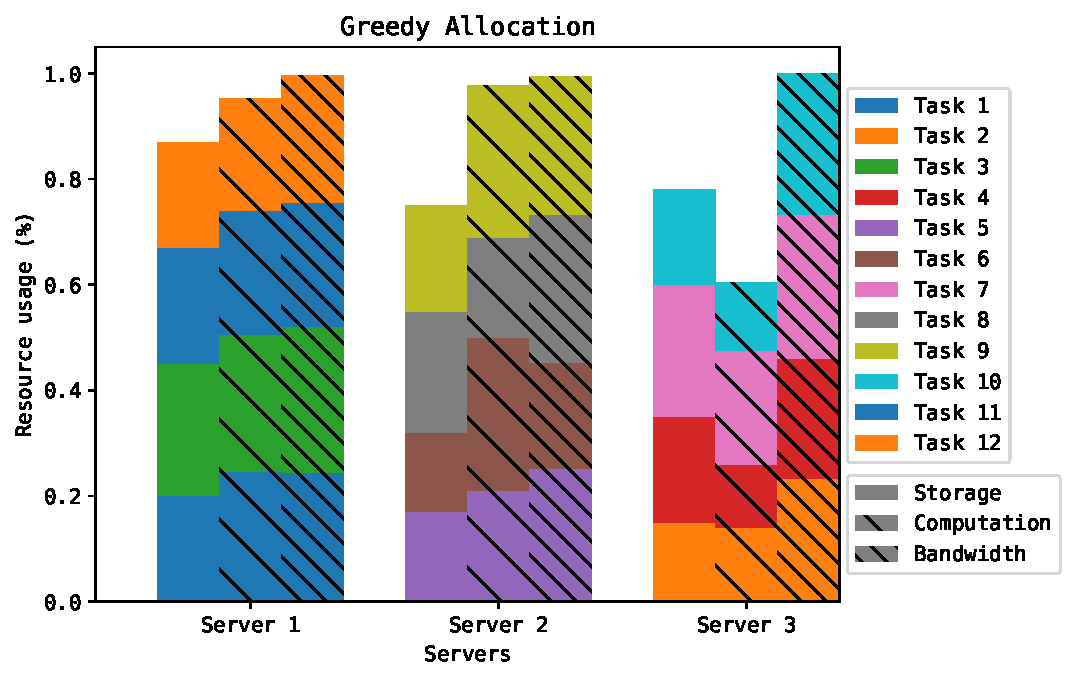
\includegraphics[width=\linewidth]{fig/allocation/greedy_allocation.pdf}
    \caption{Example Greedy allocation using model from table \ref{table:jobs} and \ref{table:servers}}
    \label{fig:greedy_allocation}
\end{figure}

\begin{algorithm}
    \caption{Pseudo code of Greedy Mechanism}
    \label{alg:greedy_mechanism}
    \begin{algorithmic}
        \REQUIRE $J$ is the set of tasks and $I$ is the set of servers
        \REQUIRE $S^{'}_i$, $W^{'}_i$ and $R^{'}_i$ is the available resources (storage, computation and bandwidth respectively) of server $i$
        \REQUIRE $\alpha(j)$ is the value density function of task $j$
        \REQUIRE $\beta(j, I)$ is the server selection function of task $j$ and set of servers $I$ returning the best server, or $\emptyset$ if the task is not able to be run on any server
        \REQUIRE $\gamma(j, i)$ is the resource allocation function of a task and server returning the loading, compute and sending speeds
        \REQUIRE $\text{sort}(X, f)$ is a function that returns a sorted list of elements in descending order, based on a set of elements $X$ and a function for comparing elements $f$

        \STATE{$J^{'} \leftarrow sort(J, \alpha)$}
        \FORALL{$j \in J^{'}$}
        \STATE{$i \leftarrow \beta(j, I)$}
        \IF{$i \neq \emptyset$}
        \STATE{$s^{'}_j, w^{'}_j, r^{'}_j \leftarrow \gamma(j, i)$}
        \STATE{$x_{i,j} \leftarrow 1$}
        \ENDIF
        \ENDFOR
    \end{algorithmic}
\end{algorithm}

Using the greedy mechanism (algorithm~\ref{alg:greedy_mechanism}), the time complexity is polynomial,
$O(\left|J\right| \left|I\right|)$.
\begin{theorem}
    Time complexity of the greedy mechanism is $O(\left|J\right| \left|I\right|)$, where $\left|J\right|$ is the number
    of tasks and $\left|I\right|$ is the number of servers. Assuming that the value density and resource allocation
    heuristics have constant time complexity and the server selection function is $O(\left|I\right|)$.
    %% TODO to check if the resource allocation heuristic is constant time complexity (KKT) probably wrong
\end{theorem}
\begin{proof}
    The time complexity of the stage 1 of the mechanism is $O(\left|J\right| \log(\left|J\right|))$ due to sorting the
    tasks and stage 2 has complexity $O(\left|J\right| \left|I\right|)$ due to looping over all of the tasks and
    applying the server selection and resource allocation heuristics. Therefore the overall time complexity is
    $O(\left|J\right| \left|I\right| + \left|J\right| \log(\left|J\right|) = O(\left|J\right| \left|I\right|)$.
\end{proof}

\subsection{Critical Value Auction}\label{subsec:critical-value-auction}
Due to the problem case being non-cooperative, if the greedy mechanism was used to allocate resources such that the
value is the price paid. This would be open to manipulation and misreporting of task attributes like the value,
deadline or resource requirements. Therefore in this section we propose an auction that is strategyproof
(weakly-dominant incentive compatible) so users have no incentive to misreport task attributes.

Single-Parameter domain auctions are extensively studied in mechanism design~\cite{nisan2007algorithmic_228} and are
used where an agent's valuation function can be represented as single value. The task price is calculated by finding
the critical value, the minimum task price required for the task to still allocated by the greedy mechanism. This has
been shown to be a strategyproof~\cite{nisan2007algorithmic_229_230} auction making it a weakly-dominant strategy for
a user to honestly reveal a task's attribute.

The auction is implemented using the greedy mechanism from section~\ref{subsec:greedy-mechanism} to find an allocation
of tasks using the reported value. The critical value for each task is found by rearranging the value density function
to makes the value the subject and the value density of the task equal to the minimum value density such the task is
still allocated in the list. Because of this, the time complexity is the same as the greedy mechanism,
$O(\left|J\right| \log(\left|J\right|))$ as it is just repeating this mechanism twice. The first to find the tasks
allocated normally with the second allocation, running through all of the tasks allocated to check the last position
in the value density list to find the position where the task couldn't be allocated on any server.

In order that the auction is strategyproof, the value density function must be
monotonic~\cite{nisan2007algorithmic_229_230} so that misreporting of any task attributes will result in the value
density decreasing. Therefore a value density function of the form $\frac{v_j d_j}{\alpha(s_j, w_j, r_j)}$ must be used so
that the auction is strategyproof.
\begin{theorem}
    The value density function $\frac{v_j d_j}{\alpha(s_j, w_j, r_j)}$ is monotonic increasing for task $j$ assuming the
    function $\alpha(s_j, w_j, r_j)$ is monotonic increasing.
\end{theorem}
\begin{proof}
    In order to misreport the task value and deadline, misreported values must be less than their true value, therefore
    if the value or deadline are decreased then the density will likewise decrease.
    While the opposite is true for the required resources (storage, compute and result data) as the misreported value
    must be greater than the true value. As the $\alpha$ function is will increase as the resource requirements increase,
    the resulting density will decrease.
\end{proof}

\subsection{Decentralised Iterative Auction}\label{subsec:decentralised-iterative-auction}
In some application of edge cloud computing, keeping the value of a task a secret is important for example
military-tactical networks. Therefore we propose a novel decentralised iterative auction based on the pricing principle
of the VCG auction~\citep{vickrey, Clarke, groves}. VCG auctions calculates the price of a tasks by finding the
difference in social welfare if the task is considered in the allocation and when the task isn't. Our proposed novel
auction uses the same principle, except without requiring a task value, by calculating a task's price by finding the
difference between the current server revenue and the revenue when the task is required to be allocated with zero value.

Our auction uses this principle by iteratively letting a task advertise its requirements to all of the servers, who
respond with their price to run the task. This price is equal to the server's current revenue minus the solution to the
problem in section~\ref{subsubsec:decentralised_iterative_problem} plus a small value referred to as the price change
variable. The reason for the price change variable is to increase the revenue of the server (otherwise the total
revenue of the server doesn't increase by accepting the task) and is be chosen by the server. Once all of the servers
have responded, the task can compare the minimum server prices to its private value. If the price is less then the
task will accept the server with the lowest price, otherwise the task must stop advertising as the price for the task
to run on any server is greater than its reserve price preventing the task from ever being allocated again.

\subsubsection{Server revenue optimisation problem}\label{subsubsec:decentralised_iterative_problem}
To find the optimal revenue for a server $m$ given a new task $n^{'}$ and set of currently allocated tasks $N$ has a
similar formulation to the optimisation problem in section~\ref{subsec:optimisation-problem}. Except with an additional
variable for the task price $p_n$ for each task $n$.

\begin{align}
    \max & \sum_{\forall n \in N} p_n x_n\label{eq:dia_objective}\\
    \mbox{s.t.} \nonumber \\
    & \sum_{\forall n \in N} s_n x_n + s_{n^{'}} \leq S_m,\label{eq:dia_server_storage_constraint}\\
    & \sum_{\forall n \in N} w^{'}_n x_n + w_{n^{'}} \leq W_m, \label{eq:dia_server_computation_constraint}\\
    & \sum_{\forall n \in N} (r^{'}_n + s^{'}_n) \cdot x_n + (r^{'}_{n^{'}} + s^{'}_{n^{'}}) \leq R_m, \label{eq:dia_server_communication_constraint}\\
    & \frac{s_n}{s^{'}_n} + \frac{w_n}{w^{'}_n} + \frac{r_n}{r^{'}_n} \leq d_n, &~ \forall n \in N \cup \{n^{'}\} \label{eq:dia_task_deadline}\\
    & 0 < s^{'}_n < \infty, &~ \forall{n \in N \cup \{n^{'}\}} \label{eq:dia_loading_speeds}\\
    & 0 < w^{'}_n < \infty, &~ \forall{n \in N \cup \{n^{'}\}} \label{eq:dia_compute_speeds}\\
    & 0 < r^{'}_n < \infty, &~ \forall{n \in N \cup \{n^{'}\}} \label{eq:dia_sending_speeds}\\
    & x_n \in \{0,1\} &~ \forall{n \in N} \label{eq:dia_job_allocation}
\end{align}

The objective (Eq.~\eqref{eq:dia_objective}) is to maximize the price of all currently allocated tasks (not including
the new task as the price is zero). The server resource capacity constraints
(Eqs.~\eqref{eq:dia_server_storage_constraint},~\eqref{eq:dia_server_computation_constraint}
and~\eqref{eq:dia_server_communication_constraint}) are similar to the constraints in the standard model set out in
section~\ref{subsec:optimisation-problem} except with the assumption that the task $n^{'}$ is running so there is no
need to consider if it is running or not. The deadline and non-negative resource speeds constraints
(\ref{eq:dia_task_deadline},~\ref{eq:dia_loading_speeds},~\ref{eq:dia_compute_speeds} and~\ref{eq:dia_sending_speeds})
are all the same equation as the standard formulation for all of the tasks plus the new task. As this formulation only
considers a single server, the task allocation constraint is not consider.

For our proposed auction, we consider four important properties in auction theory.
\begin{itemize}
    \item Budget balanced - True, since the auction can run without an auctioneer, the auction can be run in a
    decentralised system resulting in no ''middlemen'' taking some money meaning that all revenue goes straight to
    the servers from the tasks.
    \item Individually Rational - True, as the server need to confirm with the task if it is willing to pay an amount
    to be allocated, the task can check this against its secret reserved price preventing the task from ever paying
    more than it is willing.
    \item Incentive Compatible - False, as major problem for tasks is being deallocated from a server. Task can
    misreport its attribute making it cheaper for another task to be allocated to another server preventing the
    misreported task from being deallocated.
    \item Economic efficiency - False, at the beginning tasks are almost randomly assigned till servers become full and
    require kicking tasks off. This can cause the allocation to fall into a local price maxima meaning that the
    server will sometimes not be 100\% economically efficient.
\end{itemize}

The algorithm~\ref{alg:dia} is a centralised version of the auction. It works through iteratively checking a currently
unallocated job to find the price if the job was currently allocated on a server. This is done through first solving
the program in section~\ref{subsubsec:decentralised_iterative_problem} which calculates the new revenue if the task was
forced to be allocated with a price of zero. The task price is equal to the current server revenue minus the new
revenue with the task allocated plus a price change variable in order to increase the revenue of the server. The
minimum price returned by $P(i, k)$ is then compared to the job's maximum reserve price (that would be private in the
equivalent decentralised algorithm) to confirm if the job is willing to pay at that price. If the job is willing then
the job is allocated to the minimum price server and the job price set to the agreed price. However in the process of
allocating a job then the currently allocated jobs on the server could be unallocated so these jobs allocation's and
price's are reset then appended to the set of unallocated jobs.

\begin{algorithm}[H]
    \caption{Decentralised Iterative Auction}
    \label{alg:dia}
    \begin{algorithmic}
        \REQUIRE $I$ is the set of servers
        \REQUIRE $J$ is the set of unallocated tasks, which initial is the set of all tasks to be allocated
        \REQUIRE $P(i, k)$ is solution to the problem in section~\ref{subsubsec:decentralised_iterative_problem}
        using the server $i$ and new task $k$.
        The server's current tasks is known to itself and its current revenue from tasks so not passed as arguments.
        \REQUIRE $R(i, k)$ is a function returning the list of tasks not able to run if task $k$ is allocated to server $i$
        \REQUIRE $\leftarrow_R$ will randomly select an element from a set
        \WHILE{$|J| > 0$}
        \STATE{$j \leftarrow_R J$}
        \STATE{$p, i \leftarrow argmin_{i \in I} P(i, j)$}
        \IF{$p \leq v_j$}
        \STATE{$p_j \leftarrow p$}
        \STATE{$x_{i, j} \leftarrow 1$}
        \FORALL{$j^{'} \in R(i, j)$}
        \STATE{$x_{i, j^{'}} \leftarrow 0$}
        \STATE{$p_j^{'} \leftarrow 0$}
        \STATE{$J \leftarrow J \cup j^{'}$}
        \ENDFOR
        \ENDIF
        \STATE{$J \leftarrow J \setminus \{j\}$}
        \ENDWHILE
    \end{algorithmic}
\end{algorithm}

\subsection{Attributes of proposed algorithms}
In this paper, we have presented three mechanisms to solve the optimisation problem proposed in
section~\ref{subsec:optimisation-problem}. The table~\ref{tab:attributes_algorithms} considers a range of
important attributes of the proposed algorithm to allow easy comparison between the Greedy mechanism (GM),
Critical Value auction(CVA) and Decentralised Iterative auction (DIA).

\begin{table}[H]
    \centering
    \begin{tabular}{|p{2.2cm}|p{1.5cm}|p{1.5cm}|p{1.5cm}|}
        \hline
        Attribute & GM & CVA & DIA \\ \hline \hline
        Truthfulness & & Yes & No \\ \hline
        Optimality & No & No & No \\ \hline
        Scalability & Yes & Yes & No \\ \hline
        Information requirements from users & All & All & Not the reserve value \\ \hline
        Communication over heads & Low & Low & High \\ \hline
        Decentralisation & No & No & Yes \\ \hline
    \end{tabular}
    \caption{Attributes of the proposed algorithms: Greedy mechanism (GM), Critical Value auction(CVA) and Decentralised Iterative auction (DIA)}
    \label{tab:attributes_algorithms}
\end{table}
